\newcommand{\vect}[1]{\mathbf{#1}}

\item \points{12} {\bf AdaBoost}

Consider building an ensemble of decision stumps $f_t$ with the AdaBoost algorithm,
$$F(x) = \text{sign}\Big(\sum_{t=1}^T \hat{w}_t f_t(x)\Big).$$
Figure~\ref{fig:adaboost} displays a 2-dimensional training dataset, as well as the first stump chosen. A stump predicts binary $+1 / -1$ values, and depends only on one coordinate value (the split point). The little arrow indicates the positive side where the stump predicts $+1$. All points start with uniform weights.
\begin{figure}[ht]
	\centering
	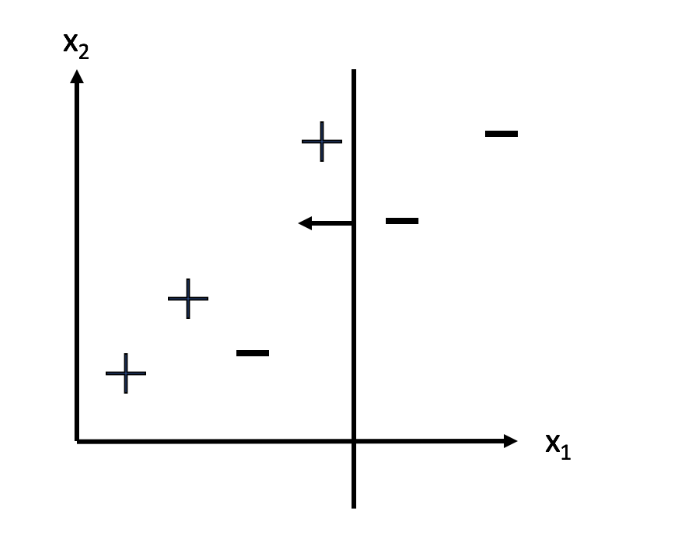
\includegraphics[width=0.45\linewidth]{adaboost/fig6-decision-boundary.png}
	\vspace{-0.1in}
	\caption{2-dimensional labeled data, where `+' corresponds to class $y=+1$ and `-' corresponds to class $y = -1$. The decision boundary for the first decision stump is shown.  The arrow points in the positive direction from this decision boundary.}
	\label{fig:adaboost}
\end{figure}

\begin{enumerate}
    \item \subquestionpoints{3} Given a set of $n$ observations $(x_i, y_i)$ where $y_i$ is the label $y_i \in \{-1,1\}$, let $f_t(x)$ be the weak classifier at step $t$ and let $\hat{w}_t$ be its weight. First we note that the final classifier after $T$ steps is defined as
		\begin{align*}
			F(x) = \text{sign} \left\{\sum_{t=1}^T \hat{w}_t f_t(x) \right\}
			= \text{sign}\{f(x)\},
		\end{align*}
	where
	\begin{align*}
		f(x) = \sum_{t=1}^T \hat{w}_t f_t(x).
	\end{align*}
	We can assume that $f(x)$ is never exactly zero.

	Show that
	\begin{align*}
		\varepsilon_{\text{training}}
		:= \frac{1}{n} \sum_{i=1}^n 1_{\{F(x_i) \neq y_i\}}
		\le \frac{1}{n} \sum_{i=1}^n \exp(-f(x_i) y_i),
	\end{align*}
	where $1_{\{F(x_i) \neq y_i\}}$ is $1$ if $F(x_i) \neq y_i$ and $0$ otherwise.
    
	\ifnum\solutions=1 {
	\begin{answer}
Type your solutions here.
\end{answer}
        } \fi
        
    \item \subquestionpoints{4} Draw  a possible stump that we could select at the next boosting iteration. You need to draw both the decision boundary and its positive orientation. The answer may not be unique and any plausible solution is acceptable.
    
	\ifnum\solutions=1 {
	\begin{answer}{
Type your solutions here.	
}
\end{answer}
        } \fi
        
    \item \subquestionpoints{9}  We showed above that training error is bounded above by $\prod_{t=1}^T Z_t$. At step $t$ the values $Z_1$, $Z_2$, $\ldots$, $Z_{t-1}$ are already fixed therefore at step $t$ we can choose $\alpha_t$ to minimize $Z_t$. Let
		\begin{align*}
			\varepsilon_t 
			= \sum_{i=1}^n \alpha_{i, t} 1_{\{f_t(x_i) \neq y_i\}}
		\end{align*}
	be the weighted training error for the weak classifier $f_t(x)$. Then we can re-write the formula for $Z_t$ as
	\begin{align*}
		Z_t = (1-\varepsilon_t) \exp(-\hat{w}_t) + \varepsilon_t \exp(\hat{w}_t).
	\end{align*}
 \begin{enumerate}
 	\item [(i)] [3 points] First find the value of  $\hat{w}_t$ that minimizes $Z_t$. Then show that the corresponding optimal value is
	\begin{align*}
		Z^{\text{opt}}_t
		= 2 \sqrt{\varepsilon_t (1-\varepsilon_t)}.
	\end{align*}
	\item [(ii)] [3 points] Assume we choose $Z_t$ this way. Then re-write $\varepsilon_t = 1/2 - \gamma_t$, where $\gamma_t > 0$ implies better than random and $\gamma_t < 0$ implies worse than random. Then show that
	\begin{align*}
		Z_t \le \exp(-2 \gamma_t^2).
	\end{align*}
	(You may want to use the fact that $\log(1 - x) \le  -x$ for $0 \le  x < 1$.)
	\item [(iii)] [3 points] Finally, show that if each classifier is better than random, i.e.,  $\gamma_t > \gamma$ for all $t$ and $\gamma > 0$, then
	\begin{align*}
			\varepsilon_{\text{training}}
		\le \exp(-2T \gamma^2),
	\end{align*}
	which shows that the training error can be made arbitrarily small with enough steps.
 \end{enumerate}
    
	\ifnum\solutions=1 {
	\begin{answer}{
Type your solutions here.
}
\end{answer}
        } \fi
        
\end{enumerate}
